% Template for PLoS
% Version 3.5 March 2018
%
% % % % % % % % % % % % % % % % % % % % % %
%
% -- IMPORTANT NOTE
%
% This template contains comments intended 
% to minimize problems and delays during our production 
% process. Please follow the template instructions
% whenever possible.
%
% % % % % % % % % % % % % % % % % % % % % % % 
%
% Once your paper is accepted for publication, 
% PLEASE REMOVE ALL TRACKED CHANGES in this file 
% and leave only the final text of your manuscript. 
% PLOS recommends the use of latexdiff to track changes during review, as this will help to maintain a clean tex file.
% Visit https://www.ctan.org/pkg/latexdiff?lang=en for info or contact us at latex@plos.org.
%
%
% There are no restrictions on package use within the LaTeX files except that 
% no packages listed in the template may be deleted.
%
% Please do not include colors or graphics in the text.
%
% The manuscript LaTeX source should be contained within a single file (do not use \input, \externaldocument, or similar commands).
%
% % % % % % % % % % % % % % % % % % % % % % %
%
% -- FIGURES AND TABLES
%
% Please include tables/figure captions directly after the paragraph where they are first cited in the text.
%
% DO NOT INCLUDE GRAPHICS IN YOUR MANUSCRIPT
% - Figures should be uploaded separately from your manuscript file. 
% - Figures generated using LaTeX should be extracted and removed from the PDF before submission. 
% - Figures containing multiple panels/subfigures must be combined into one image file before submission.
% For figure citations, please use "Fig" instead of "Figure".
% See http://journals.plos.org/plosone/s/figures for PLOS figure guidelines.
%
% Tables should be cell-based and may not contain:
% - spacing/line breaks within cells to alter layout or alignment
% - do not nest tabular environments (no tabular environments within tabular environments)
% - no graphics or colored text (cell background color/shading OK)
% See http://journals.plos.org/plosone/s/tables for table guidelines.
%
% For tables that exceed the width of the text column, use the adjustwidth environment as illustrated in the example table in text below.
%
% % % % % % % % % % % % % % % % % % % % % % % %
%
% -- EQUATIONS, MATH SYMBOLS, SUBSCRIPTS, AND SUPERSCRIPTS
%
% IMPORTANT
% Below are a few tips to help format your equations and other special characters according to our specifications. For more tips to help reduce the possibility of formatting errors during conversion, please see our LaTeX guidelines at http://journals.plos.org/plosone/s/latex
%
% For inline equations, please be sure to include all portions of an equation in the math environment.  For example, x$^2$ is incorrect; this should be formatted as $x^2$ (or $\mathrm{x}^2$ if the romanized font is desired).
%
% Do not include text that is not math in the math environment. For example, CO2 should be written as CO\textsubscript{2} instead of CO$_2$.
%
% Please add line breaks to long display equations when possible in order to fit size of the column. 
%
% For inline equations, please do not include punctuation (commas, etc) within the math environment unless this is part of the equation.
%
% When adding superscript or subscripts outside of brackets/braces, please group using {}.  For example, change "[U(D,E,\gamma)]^2" to "{[U(D,E,\gamma)]}^2". 
%
% Do not use \cal for caligraphic font.  Instead, use \mathcal{}
%
% % % % % % % % % % % % % % % % % % % % % % % % 
%
% Please contact latex@plos.org with any questions.
%
% % % % % % % % % % % % % % % % % % % % % % % %

\documentclass[10pt,letterpaper]{article}
\usepackage[top=0.85in,left=2.75in,footskip=0.75in]{geometry}
%\documentclass[10pt]{article}
%\usepackage[margin=2cm]{geometry}

% amsmath and amssymb packages, useful for mathematical formulas and symbols
\usepackage{amsmath,amssymb}

% Use adjustwidth environment to exceed column width (see example table in text)
\usepackage{changepage}

% Use Unicode characters when possible
\usepackage[utf8x]{inputenc}

% textcomp package and marvosym package for additional characters
\usepackage{textcomp,marvosym}

% cite package, to clean up citations in the main text. Do not remove.
\usepackage{cite}

% Use nameref to cite supporting information files (see Supporting Information section for more info)
\usepackage{nameref,hyperref}

% line numbers
\usepackage[right]{lineno}

% ligatures disabled
\usepackage{microtype}
\DisableLigatures[f]{encoding = *, family = * }

% color can be used to apply background shading to table cells only
\usepackage[table]{xcolor}

% array package and thick rules for tables
\usepackage{array}

% create "+" rule type for thick vertical lines
\newcolumntype{+}{!{\vrule width 2pt}}

% create \thickcline for thick horizontal lines of variable length
\newlength\savedwidth
\newcommand\thickcline[1]{%
  \noalign{\global\savedwidth\arrayrulewidth\global\arrayrulewidth 2pt}%
  \cline{#1}%
  \noalign{\vskip\arrayrulewidth}%
  \noalign{\global\arrayrulewidth\savedwidth}%
}

% \thickhline command for thick horizontal lines that span the table
\newcommand\thickhline{\noalign{\global\savedwidth\arrayrulewidth\global\arrayrulewidth 2pt}%
\hline
\noalign{\global\arrayrulewidth\savedwidth}}


% Remove comment for double spacing
\usepackage{setspace} 
\doublespacing

% Text layout
\raggedright
\setlength{\parindent}{0.5cm}
\textwidth 5.25in 
\textheight 8.75in

% Bold the 'Figure #' in the caption and separate it from the title/caption with a period
% Captions will be left justified
\usepackage[aboveskip=1pt,labelfont=bf,labelsep=period,justification=raggedright,singlelinecheck=off]{caption}
\renewcommand{\figurename}{Fig}

% Use the PLoS provided BiBTeX style
\bibliographystyle{plos2015}

% Remove brackets from numbering in List of References
\makeatletter
\renewcommand{\@biblabel}[1]{\quad#1.}
\makeatother



% Header and Footer with logo
\usepackage{lastpage,fancyhdr,graphicx}
\usepackage{epstopdf}
\pagestyle{myheadings}
\pagestyle{fancy}
\fancyhf{}
\setlength{\headheight}{27.023pt}
%\lhead{\includegraphics[width=2.0in]{PLOS-submission.eps}}
\rfoot{\thepage/\pageref{LastPage}}
\renewcommand{\headrulewidth}{0pt}
\renewcommand{\footrule}{\hrule height 2pt \vspace{2mm}}
\fancyheadoffset[L]{2.25in}
\fancyfootoffset[L]{2.25in}
\lfoot{\today}

%% Include all macros below

\newcommand{\lorem}{{\bf LOREM}}
\newcommand{\ipsum}{{\bf IPSUM}}

%% END MACROS SECTION


\begin{document}
\vspace*{0.2in}

% Title must be 250 characters or less.
\begin{flushleft}
{\Large
\textbf\newline{A comparison of simple models for urban morphogenesis} % Please use "sentence case" for title and headings (capitalize only the first word in a title (or heading), the first word in a subtitle (or subheading), and any proper nouns).
}
\newline
% Insert author names, affiliations and corresponding author email (do not include titles, positions, or degrees).
\\
Juste Raimbault\textsuperscript{1,2,3,*}
\bigskip\\
\textsuperscript{1} Center for Advanced Spatial Analysis, University College London
\\
\textsuperscript{2} UPS CNRS 3611 ISC-PIF
\\
\textsuperscript{3} UMR CNRS 8504 G{\'e}ographie-cit{\'e}s
\bigskip\\
* juste.raimbault@polytechnique.edu



\end{flushleft}

% Please keep the abstract below 300 words
\section*{Abstract}
\vspace{1cm}
The spatial distribution of population and activities within urban areas, or urban form at the mesoscopic scale, is the outcome of multiple antagonist processes. We propose in this paper to benchmark different models of urban morphogenesis, to systematically compare the urban forms they can produce. Different types of approaches are included, such as a reaction-diffusion model, a gravity-based model, and correlated percolation. Applying a diversity search algorithm, we estimate the feasible space of each model within a space of urban form indicators, in comparison of empirical values for worldwide urban areas. We find a complementarity of the different types of processes, advocating for a plurality of urban models.

% urban morphogenesis; reaction-diffusion; correlated percolation; gravity model; novelty search


\linenumbers

\cite{xu2021emergence}

\cite{strano2021agglomeration}

\cite{Rybski2021Modeling} coupling inside model - more to benchmark - multimodeling

\cite{bithellsystematic} benchmark abm covid

\cite{jun2020modling} entropy and urban growth


\cite{Nicholse2100769118} reproducibility - benchmarks - sequence of studies


\section*{Introduction}

% urban form and sustainability - urban form at the mesoscopic scale

Understanding the dynamics of cities is an increasing issue for sustainability, since the proportion of the world population expected to live in cities will grow to a large majority in the next decades, and that cities combine both positive and negative externalities on most aspects. Their complexity implies that quantitative and qualitative predictions are not relevant, but planners can \emph{invent future cities} \cite{batty2018inventing}, what requires though a knowledge of key urban processes which can be acted upon. In that context, the growth of \emph{urban form} in its different definition and scales, is essential \cite{williams2000achieving}. Considering urban form at a mesoscopic scale, i.e. roughly the scale of urban areas, it can be understood as the spatial distribution of activities. More particularly the distribution of population density has a strong impact on commuting, energy consumption and emissions \cite{le2012urban}. Being able to link microscopic processes with the growth of different types of urban form is thus important for a long term planning of sustainable urban systems.

% broad overview of approaches: CA, LUTI. why study simple models (include studied models)

Urban modeling at the mesoscopic scale is the subject of diverse approaches and disciplines. Intra-urban urban economic models, building on classic works such as the Alonso-Mills-Muth model or the Fujita-Ogawa model, propose models linking land-use with land and building markets, which are spatially explicit to different degrees \cite{viguie2012trade}. Transportation and Urban Planning also have a long history in urban dynamics models, including Land-use transport interaction models \cite{wegener2004land}. Spatial interaction models can also be used in a similar manner to study urban dynamics and as a by-product urban form \cite{milton2019accelerating}. Cellular automata models of urban growth are also a privileged approach to study the growth of urban form from a data-driven perspective \cite{batty1997cellular}.

At the interface of physics, artificial life and quantitative geography, a few approaches propose simple models to explain the growth of urban form, and generally rely on an unidimensional description of urban form, namely the distribution of population or of the built environment. In that context, the correlated percolation model introduced by \cite{makse1998modeling} was a precursor. Such models can rely on abstract physical processes but also on agent behavior, such as in the Sugarscape model which according to \cite{batty2007cities} can be considered as a model for human settlements. \cite{murcio2015urban} use migration between cities at multiple scales to simulate urban growth. Diffusion-limited aggregation (DLA) is an other approach transferred from physics to urban modeling \cite{batty1989urban} and has shown relevant to reproduce fractal urban structures and urban migration processes \cite{murcio2009colored}. \cite{murcio2013second} combines DLA with percolation to obtain more realistic urban forms. Closer to the idea of urban morphogenesis, \cite{10.1371/journal.pone.0203516} proposes a reaction-diffusion model to capture fundamental urban growth processes. \cite{li2019singularity} describes an urban growth model based on geographical processes, namely an aggregation of population driven by spatial interaction. All these works have in common to model urban growth in synthetic settings, at a mesoscopic scale, considering population distribution only, and in a stylized way. They furthermore consider diverse processes, remaining simple in their structure although they lead to the emergence of a complex behavior. We will in this paper focus on such models, referring to them as \emph{models of urban morphogenesis}.

% urban multi-modeling/multidimensionality: importance of plurality of views: why benchmark

Exhibiting models with a few number of parameters and processes is useful from an explanative viewpoint, when these can reproduce real world configurations. Having multiple concurrent models which include diverse, complementary or contradictory processes, is furthermore useful for the construction of integrated urban theories, since concurrent explanations can be benchmarked, compared and possibly integrated into multi-modeling approaches. This plurality in urban modeling is intrinsic to a literature with multiple disciplines focusing on a same object of study \cite{pumain2020conclusion}.


% research question / contributions

We propose thus in this paper to benchmark several simple models of urban morphogenesis, in order to understand the potentialities of some of these models to exhibit a complex behavior and reproduce existing urban forms, and compare them in a systematic way. More precisely, our contributions are the following: (i) we integrate four different models (correlated percolation, reaction-diffusion, gravity and exponential mixture) into a single software framework; (ii) we compute measures of urban form for urban areas worldwide; (iii) we apply a novelty search algorithm to the models in order to determine their feasible morphological space, and compare these to real urban form values. This contributes to a general understanding of the complementarity of urban models, more particularly for urban morphogenesis at this scale.


% organization

The rest of this paper is organized as follows: we first describe the models benchmarked and the quantitative measures used for urban form; we describe empirical values of urban morphology indicators for urban areas worldwide; these are then compared to the feasible space of each model obtained with a diversity search algorithm. We finally discuss the implications of these results for theories of urban morphogenesis and possible developments.



\section*{Materials and methods}

%\subsection*{Processes}
% kind of systematic review of possibly involved processes?

\subsection*{Urban morphogenesis models}

We study and compare four different models of urban morphogenesis. We consider a population grid of size $N = W\times H$ (not necessarily square), each cell being characterized by its population $P_i$ with $1\leq i \leq N$.

\subsubsection*{Gravity-based model}

% modified: exponent for spatial interaction model; multiple seeds (polycentricity)

Following the so-called ``first law of geography'', entities in space have interaction patterns which can be described with spatial interaction models \cite{fotheringham1989spatial}, including the gravity model. \cite{li2019singularity} proposed an urban growth model including this process within an iterative growth with population aggregation processes, extending a more simple model introduced by \cite{rybski2013distance}. We generalize this model by adding (i) a hierarchy parameter regarding population aggregation and (ii) seeding multiple initial sites to allow the emergence of polycentric urban forms.

Formally, an initial grid is seeded with $P_0^{(G)}$ sites with population 1, randomly selected. Then, iteratively, one unit of population is added to each cell at each time step with a probability proportional to 
\begin{equation}
p_i \propto \frac{\sum_{j\neq i} P_j^{\gamma_P^{(G)}} \cdot d_{ij}^{- \gamma_D^{(G)}}}{\sum d_{ij}^{- \gamma_D^{(G)}}}
\end{equation}

where probabilities are rescaled such that the cell with the larger value has a probability of $g^{(G)}$. This last parameter allows modifying the speed of growth. The model is stopped when a total population $P_M^{(G)}$ is reached.

\subsubsection*{Reaction-diffusion}

% modify: max density? - NO

In his attempt to understand embryogenesis, Alan Turing proposed to use chemical partial differential equations (PDEs) to model morphogenesis, introducing the nowadays famous reaction-diffusion equations \cite{turing1990chemical}. In such systems, chemical substances react together and diffuse in space, leading to the emergence of complex geometrical patterns. The concept of morphogenesis has been since well used in urban studies \cite{raimbault2018co}, but very few models have actually implemented reaction-diffusion equations, \cite{bonin2014modelisation} being a notable exception. \cite{10.1371/journal.pone.0203516} proposes to capture the fundamental processes of agglomeration economies (positive externalities) leading to aggregation and of congestion (negative externalities) leading to sprawl, as an ``aggregation-diffusion'' model of urban morphogenesis. The model yields indeed in certain limits reaction-diffusion PDEs. Formally, starting from an empty grid, $N^{(R)}$ units of population are added at each time step, and attributed independently to cells with a probability proportional to $P_i^{\alpha^{(R)}}$ (probabilities are rescaled to obtain a probability distribution over all cells). Population is then diffused in space $d^{(R)}$ times with a strength $\beta^{(R)}$. The model is stopped when a maximum population $P_M^{(R)}$ is reached.



\subsubsection*{Correlated percolation}

The first two models presented are iterative and can in theory be used dynamically. Other approaches, closer to procedural modeling \cite{parish2001procedural}, do not simulate the progressive growth of population. They can however capture processes at play in the growth of urban form. The correlated percolation model described by \cite{makse1998modeling} integrates for example clustering processes in cities. A method to generate a spatial field exhibiting long range correlations was introduced for problems in physics by \cite{makse1996method}. It is combined to a monocentric density profile in \cite{makse1998modeling} to produce urban forms. In practice, a correlated field $p_i$ is generated by (i) generating a random spatial field; (ii) compute its spatial Fourier transform; (iii) introduce a correlation by multiplying it with a spectral density function with a power-law exponent $\alpha^{(C)}$; (iv) retrieve a long-range correlated spatial field by taking the inverse Fourier transform. This field is combined to a density field $\rho_i$ to determine a binary value for the cell: it is populated if $p_i > \theta_i$ with $\rho_i = \int_{-\infty}^{\theta_i} d\mathbb{P}(p_i)$. We generalize the initial model by taking a polycentric density field with 

\begin{equation}
\rho_i (\vec{x}) = \sum_{j=1}^{n^{(C)}} \exp\left(\lVert\vec{x} - \vec{x}_j\rVert / r_j\right)
\label{eq:kernelmixture}
\end{equation}

where the kernel centers are chosen at random and kernel sizes $r_j$ are taken such that kernel populations follow a rank-size law of hierarchy $\beta^{(C)}$ and the largest kernel has a fixed size $r_0^{(C)}$.

\subsubsection*{Kernel mixtures}

Finally, to provide some kind of null model to understand the advantages of each approach compared to a simple description of population distribution, we also include urban forms generated as kernel mixtures. We consider in particular exponential mixtures \cite{anas1998urban}, where population density is written as previously in Eq.~\ref{eq:kernelmixture}. Parameters for this model are the number of kernels $n^{(E)}$, the rank-size hierarchy $\alpha^{(E)}$, the size of the largest kernel $r_0^{E}$. Contrary to previous models in which total population had an influence by controlling the speed of growth, density can here be rescaled arbitrarily (morphological indicators used are not changed through rescaling, see below), and we set the maximal density for one kernel to one.


% null model: white noise? (for robustness of indicators)



\subsection*{Measures of urban form}

% already computed for dynamical calib for world urban areas -> use same measures. todo future work: benchmark measures world areas: landscape eco, etc.

Quantitative measures of urban form are multiple and depend on the scale considered \cite{zhang2005metrics}. \cite{raimbault2019generating} for example introduces measures for buildings at the district scale. The field of Landscape Ecology has its own metrics similar to urban form measures \cite{10.1371/journal.pone.0225734}. For the scale we consider and considering population distribution only, metrics of urban form have been proposed for example to quantify sprawl \cite{tsai2005quantifying}. These can be related to fractal approaches to urban form \cite{chen2011derivation}. The effective dimension when applied to real cities is reasonably low \cite{schwarz2010urban}, and a few complementary indicators can be used. We thus follow \cite{10.1371/journal.pone.0203516} and consider urban form measures which are: (i) Moran index to capture spatial autocorrelation and the existence of centers; (ii) average distance between individuals which captures a level of aggregation; (iii) distribution entropy (aspatial) to capture the uniformity of the distribution; and (iv) rank-size slope which captures the hierarchy of population distribution.






\section*{Results}


\subsection*{Implementation}

The models are implemented in \texttt{scala} and integrated into the \texttt{spatialdata} library for spatial sensitivity analysis \cite{raimbault2020scala}. The library is bundled as an OpenMOLE plugin for the numerical experiments. OpenMOLE is an open source software for model exploration and validation \cite{reuillon2013openmole} combining model embedding with state-of-the-art exploration methods (including for example sensitivity analysis, design of experiments, calibration with genetic algorithms) and a transparent distribution of computations on high performance computing environments. In our case, we use its workflow system and an integrated algorithm to determine the feasible space of models. Source code for models is available in the open source code of the \texttt{spatialdata} library at \url{https://github.com/openmole/spatialdata}. Source code for numerical experiments, simulation data and results used in this paper are available on an open git repository at \url{https://github.com/JusteRaimbault/UrbanGrowth}. Full simulation data is available on the dataverse repository at \url{https://doi.org/10.7910/DVN/VVIEYO}.



\subsection*{Empirical data}



%%%%%%%%%%%%%%
\begin{figure}[!h]
	%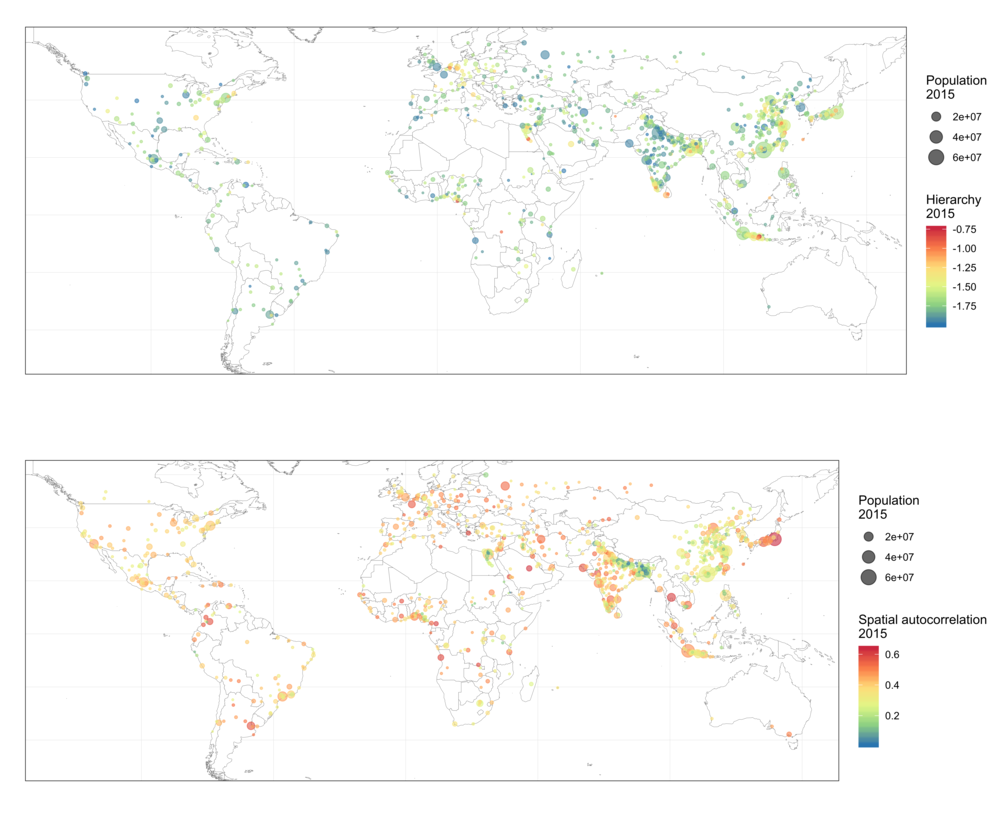
\includegraphics[width=\linewidth]{figures/Fig1.png}
	\vspace{2cm}
	\caption{{\bf Maps of urban morphology indicators for worldwide urban areas.} (Top) Rank-size hierarchy; (Bottom) Moran spatial autocorrelation index. Area of circles gives population.\label{fig:fig1}}
% TODO redo maps with open resources https://www.naturalearthdata.com/downloads/110m-cultural-vectors/
\end{figure}
%%%%%%%%%%%%%%


%%%%%%%%%%%%%%
\begin{figure}[!h]
	%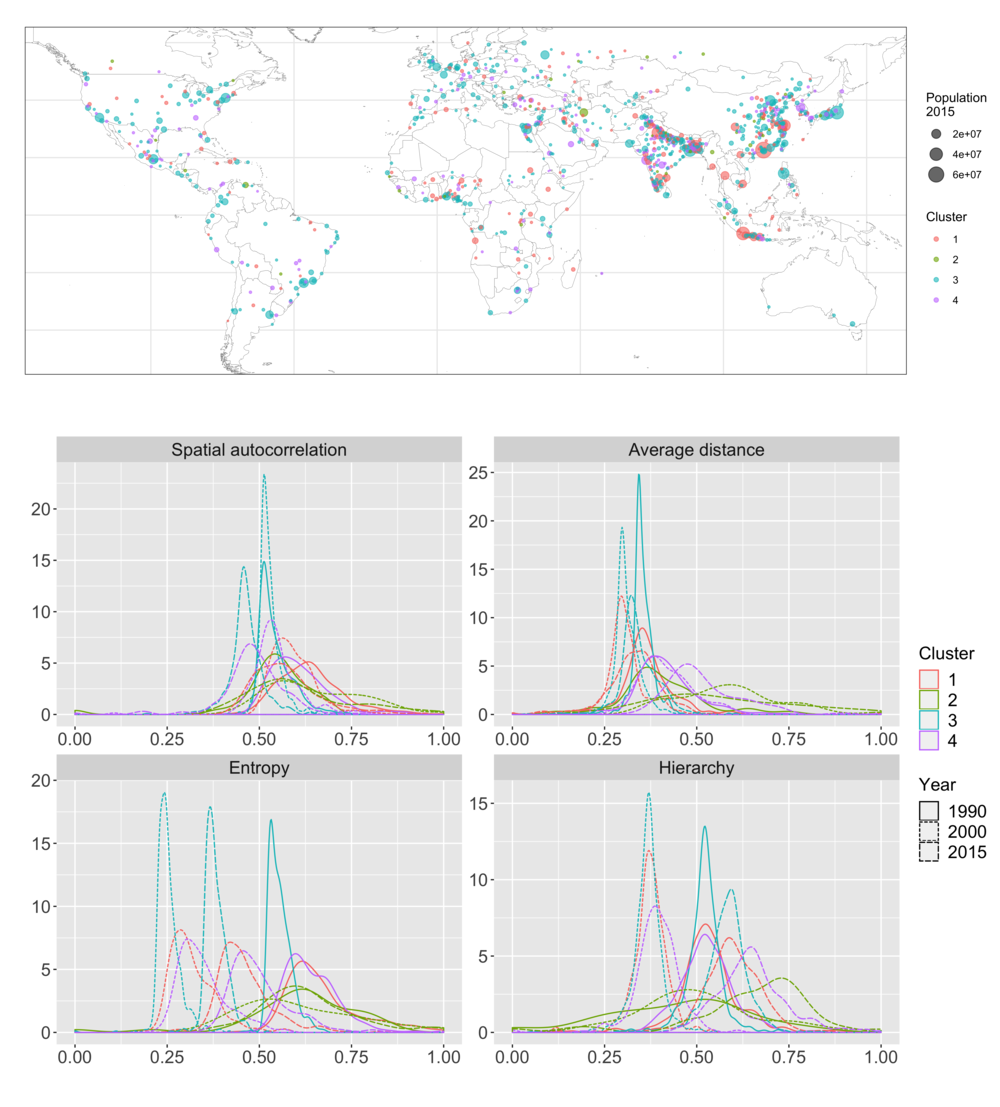
\includegraphics[width=\linewidth]{figures/Fig2.png}
	\vspace{2cm}
	\caption{{\bf Urban form typology. Using an unsupervised k-means clustering algorithm, we find clusters among urban areas.} (Top) Map of cluster belonging; (Bottom) Statistical distribution of indicator values, within each cluster and in time for all dates in the GHSL dataset.\label{fig:fig2}}
\end{figure}
%%%%%%%%%%%%%%

We compare model simulation results to urban form measures computed on worldwide urban areas. We use therefore the Global Human Settlement Layer database (GHSL), which provides an exhaustive worldwide population raster with a 1km resolution \cite{melchiorri2018unveiling}. \cite{Raimbault_2020} has shown the relevance of using this database for worldwide simulation models. It is available at four dates from 1975 onwards, but as not all models are dynamical we use the most recent population configuration only (2015). The database provides a layer of urban areas, within which we extract for the 1000 largest areas in terms of population a covering window ($\pm 25\%$ of extent on each side) from the population raster (note that some windows may be overlapping, as in the case of Hong-Kong which is separated from the main cluster of the Pearl River Delta mega-city region). Morphological indicators are computed on these extracted areas.

We show in Fig.~\ref{fig:fig1} maps of indicators. More particularly, we map the rank-size hierarchy and Moran spatial autocorrelation which have meaningful geographical variations. Rank-size hierarchy will tell if the metropolitan area is strongly dominated by one center or if it more balanced. We retrieve the fact that in Europe, Paris and London are known for such a strong monocentricity, compared to cities in Germany for example. Similarly, mega-city regions in East Asia (Pearl River delta, Yangtze River delta, Beijing-Tianjin) are more polycentric and thus balanced than Wuhan or Seoul. Regarding spatial autocorrelation, we also observe a strong variation in East Asia (Tokyo compared to Chinese megacities for example), and within India (agglomerations in the Gange plain making a cluster of non-correlated, thus highly sprawled areas).

The areas can be clustered following a non-supervised approach. We proceed to a k-means clustering on normalized indicator values, and find $k=4$ clusters as meaningful regarding the derivative of within-cluster variance. A map of cluster belonging and cluster profiles are shown in Fig.~\ref{fig:fig2}. We retrieve the variation within East Asia (Tokyo, Seoul and Shanghai being each in a different cluster) but less in Europe. The main cluster (light blue) corresponds to strongly monocentric urban areas. We see in density distributions of indicator values that clusters have clearly different profiles, which correspond to different typologies of urban morphology that the models try to approximate. For example, cluster 3 (light blue) and 1 (red) have the same level of hierarchy, but the latter has a much higher autocorrelation and entropy, and corresponds thus to more polycentric configurations.



%\subsection*{Behavior of models}
% also saltelli?




%%%%%%%%%%%%%%
\begin{figure}[!h]
	%
\includegraphics[width=\linewidth]{figures/Fig3.png}
	\vspace{2cm}
	\caption{{\bf Examples of generated urban forms for a square world of width $W = 50$.} From Left to Right and Top to Bottom: (i) Correlated percolation model for $r_0^{(C)} = 50$, $\alpha^{(C)} = 0.4$, $n^{(C)} = 3$; (ii) Exponential mixture model for $n^{(E)} = 10$, $r_0^{(E)} = 40$, $\alpha^{(E)} = 1$; (iii) Gravity model for $g^{(G)} = 0.3$, $\gamma_D^{(G)} = 2.5$, $\gamma_P^{(G)} = 0.5$, $P_0^{(G)} = 3$, $P_M^{(G)} = 20000$; (iv) Reaction-diffusion model for $\alpha^{(R)} = 0.8$, $\beta^{(R)} = 0.2$, $d^{(R)} = 1$, $N^{(R)} = 100$, $P_M^{(R)} = 5000$.\label{fig:fig3}}
\end{figure}
%%%%%%%%%%%%%%


\subsection*{Generated urban forms}

% examples for each model


We show in Fig.~\ref{fig:fig3} examples of generated urban forms for each model included in this study. Visually, these urban form look rather different. To what extent they are statistically distant for the morphology indicators can only be determined by systematic experiments. The gravity and percolation results look similar, although at a slightly different scale. This particular configuration of the reaction-diffusion model corresponds more to a rural or peri-urban configuration, while the exponential mixture is fuzzy and would resemble a blurred polycentric urban configuration.



%%%%%%%%%%%%%%
\begin{figure}[!h]
	%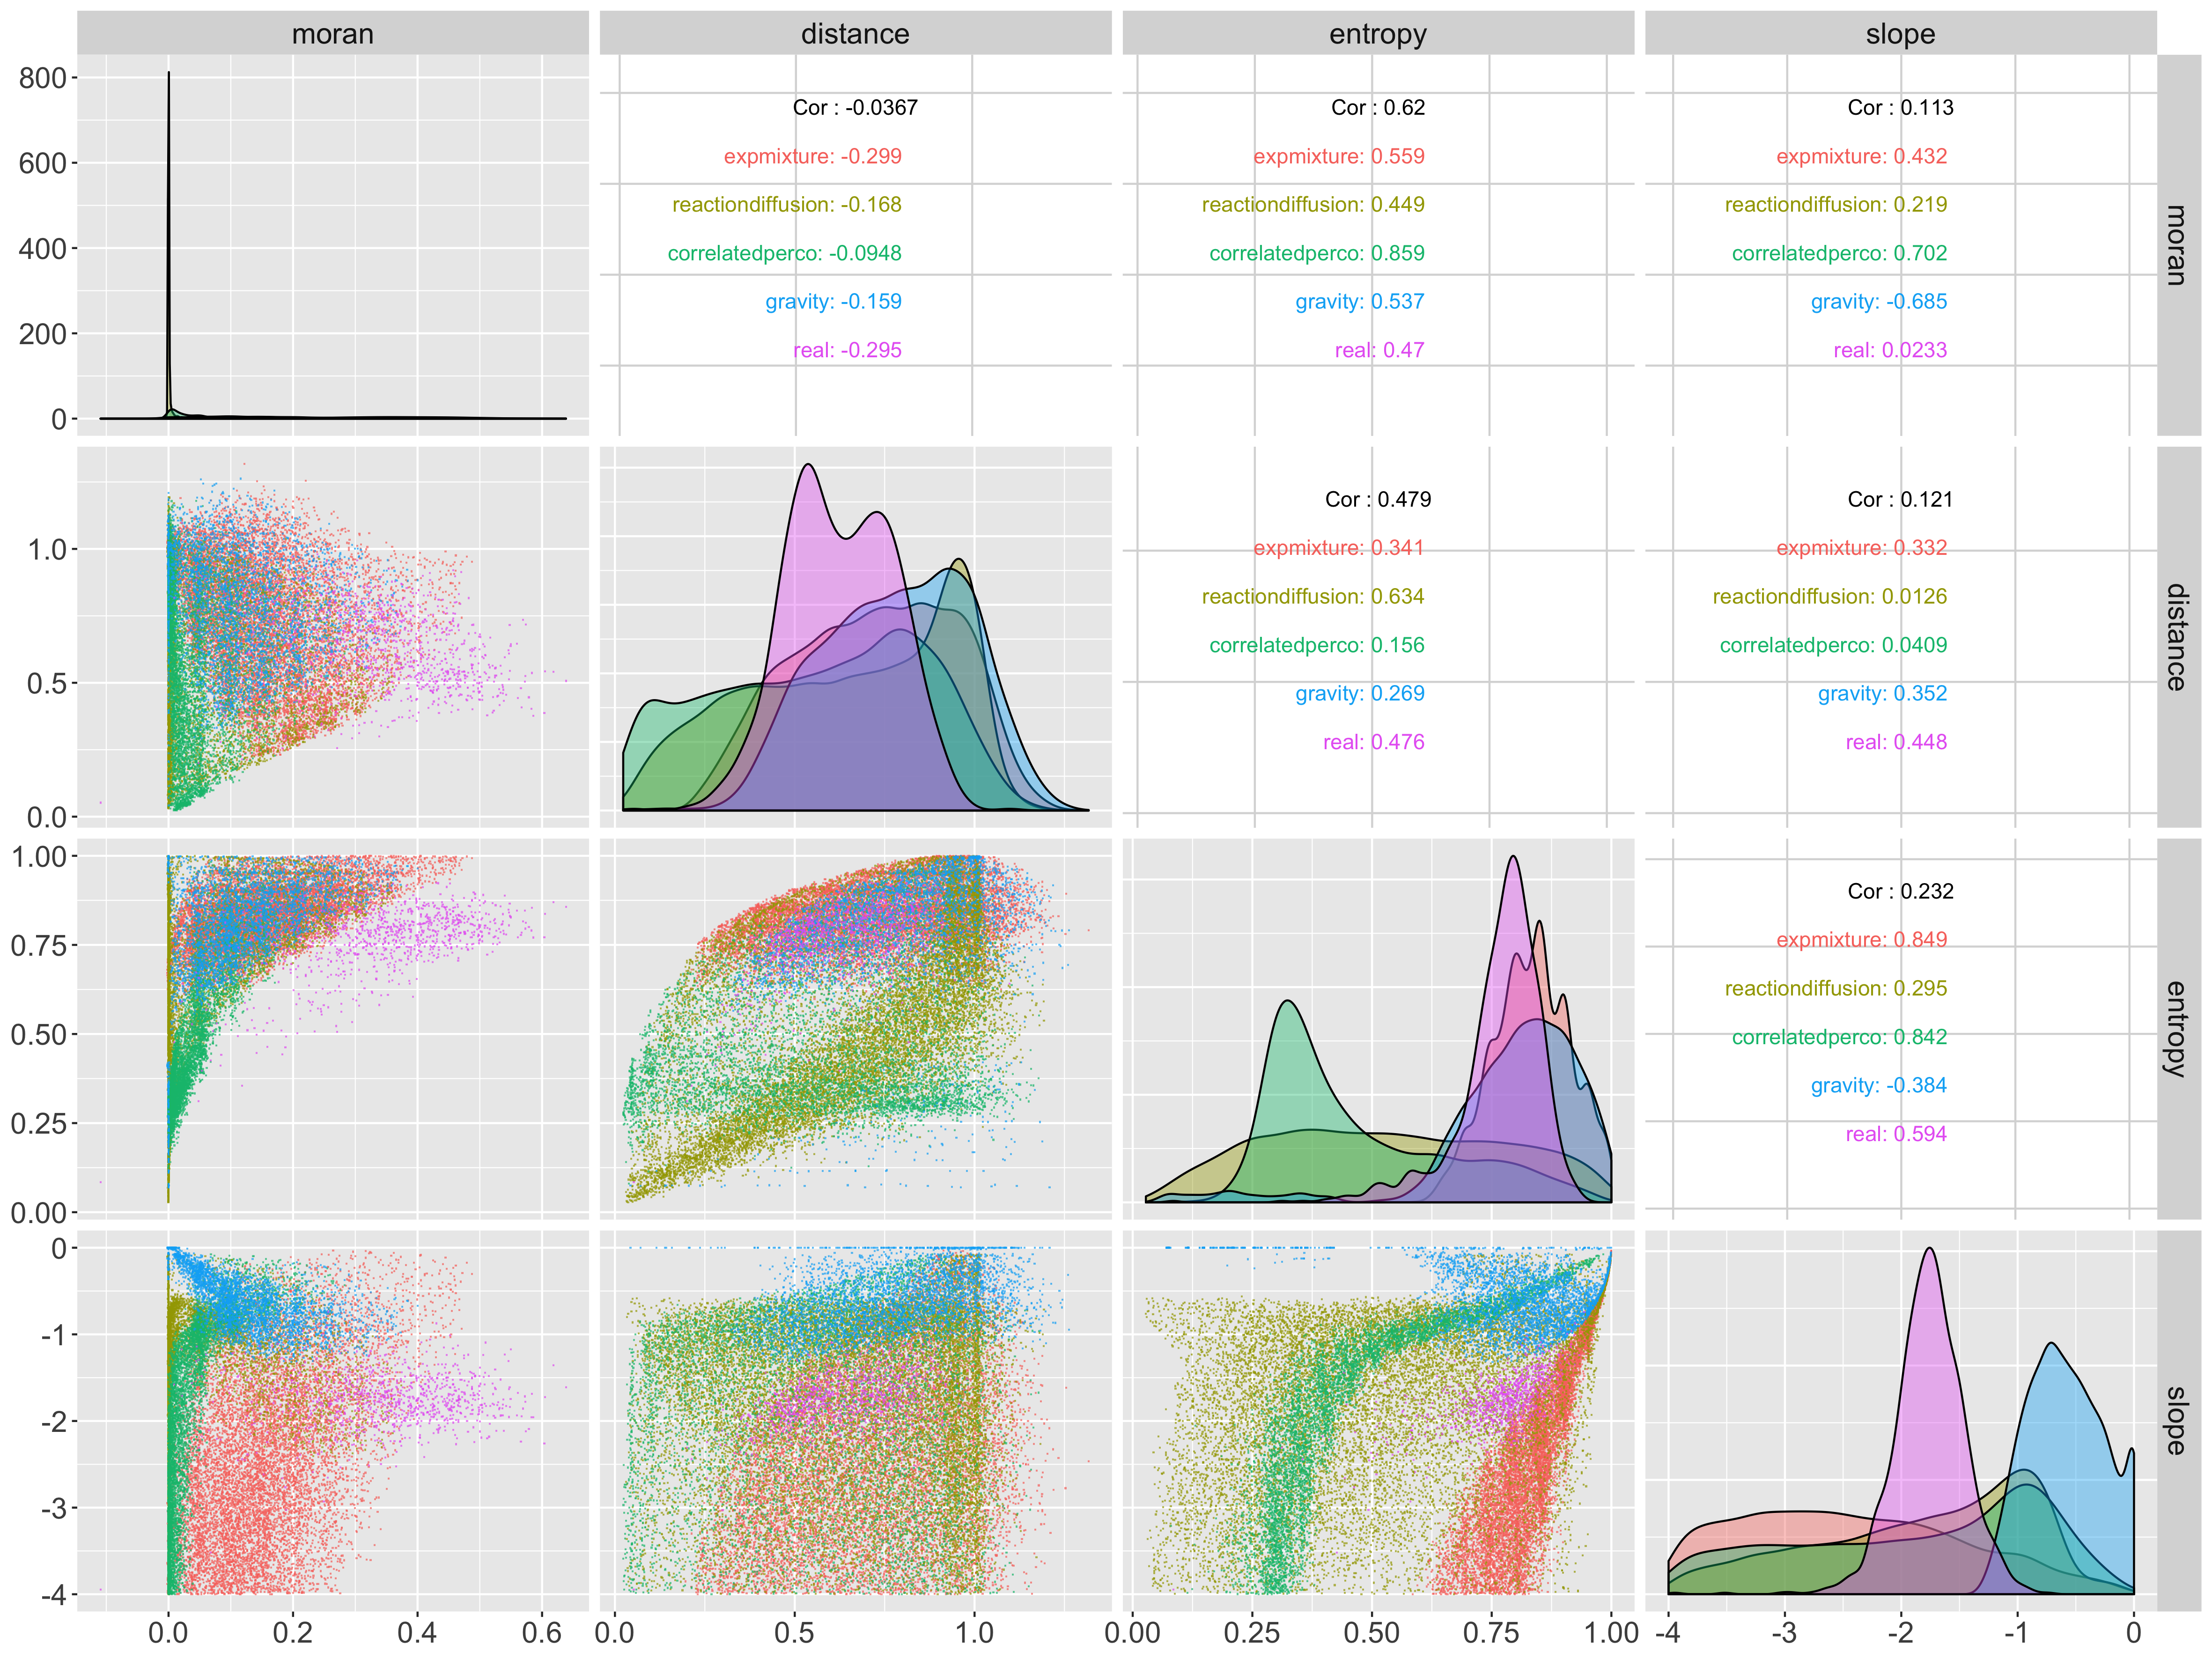
\includegraphics[width=\linewidth]{figures/Fig4.png}
	\vspace{2cm}
	\caption{{\bf Feasible morphological space for each simulation model.} The lower part of the plot matrix gives a scatterplot between each indicator. We also plot real urban areas in purple. The diagonal gives statistical distribution, while the correlation matrix is given in the upper part, conditionally to each model.\label{fig:fig4}}
\end{figure}
%%%%%%%%%%%%%%

\subsection*{Feasible morphological spaces}

We now turn to the main experiment of this paper: using a diversity search algorithm to determine the full feasible morphological space for each model. Therefore, we use the Pattern Space Exploration (PSE) algorithm \cite{cherel2015beyond} embedded in OpenMOLE. Diversity search was introduced in the field of artificial life as genetic algorithms with the aim to maximize diversity of the population \cite{lehman2008exploiting}. In the case of the PSE algorithm, a novelty criteria leads the search towards new regions of the indicator space, and results are stored in a hitmap. When running long enough, convergence in terms of number of solutions found is generally reached, and one can consider the final population as the feasible space of the model. We run here the algorithm up to 100,000 generations for each model, with grid of step 0.05 in the indicator space. Convergence was reached separately for each model.
% equivalent in terms of Islands generation?
% which spatialdata commit? 4ef6bc7c4e7887bb35138773ae87b158e6e9a19b
% (replace plugin on myoml-27/08 16h52 + remove urbgrowth acc)
% latest 36fb676ce20f1ca6586defb9f8a15ea2a366477b
% (remove urbanevolution_2.12 29/04 15:03: pb compat) (remove saltelli exec - time ok)(remove zombiesbundle 31/08 9:55)

We show in Fig~\ref{fig:fig4} a scatterplot of the final population in the morphological space. First of all, we observe that correlation are very different for each model (for example opposite value for gravity and reaction-diffusion between entropy and slope), confirming that the way urban form is produced is very different although the final form may be the same. Then, we observe that the point clouds slightly intersect but also have their own proper space that which no other model can reach. For example, in the entropy-slope space, the reaction-diffusion model is very flexible and covers a large part of space, while gravity is restricted to a small region and correlated percolation and exponential mixture exhibit much less variability with a strong correlation between the two dimensions. The models cover a similar region for the Moran-entropy space, but all fail to capture an important part of real points (in purple), corresponding to configurations with a high Moran index but a relatively low entropy. Models systematically associate a high moran with a high entropy. In other dimensions, real points are reasonably covered. Thus, we can conclude that (i) the different models are complementary in terms of urban forms produced and (ii) that a part of real configurations are approached by some of the models, but other can not be reproduced.

%%%%%%%%%%%%%%
\begin{figure}[!h]
	%\begin{center}
	%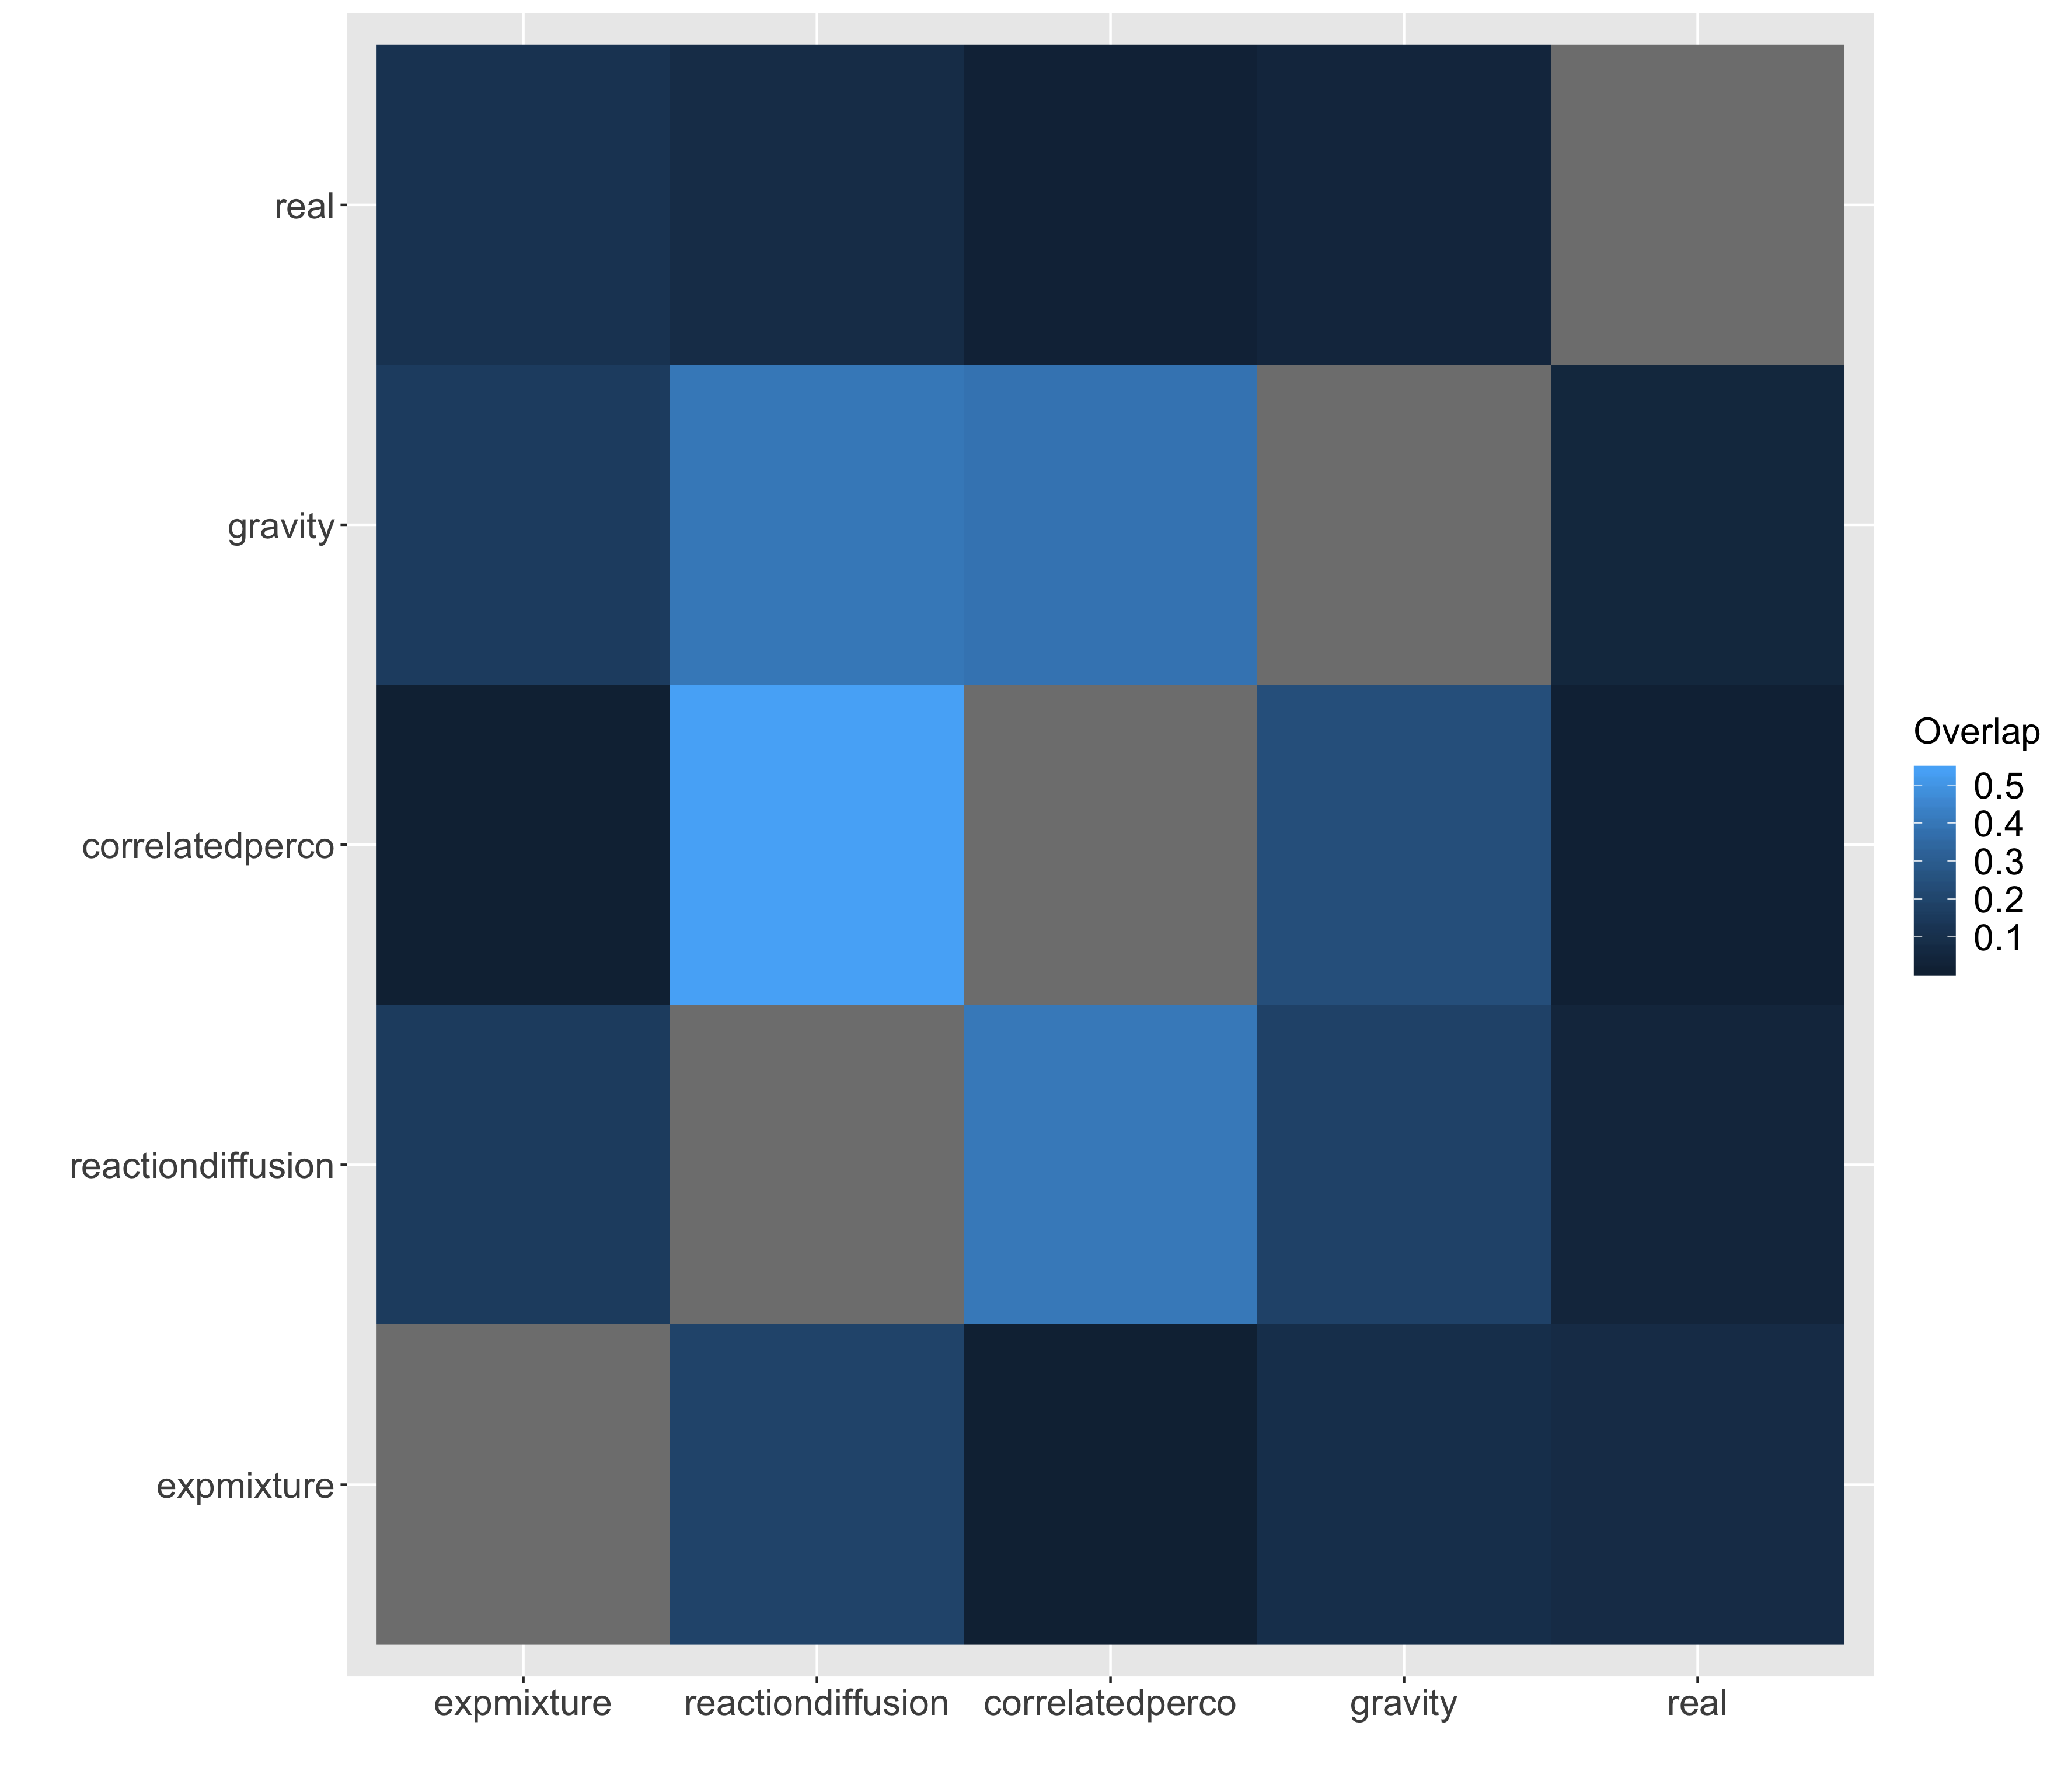
\includegraphics[width=0.6\linewidth]{figures/Fig5.png}
	%\end{center}
	\vspace{2cm}
	\caption{{\bf Overlap between point cloud hypervolumes.}\label{fig:fig5}}
\end{figure}
%%%%%%%%%%%%%%


Correlations/PCA for each model and for all points? (plus analysis in link to params? not possible in stoch? (does replication strain params? Y!)


To better quantify how each model are similar and how they approach real configurations, we compute the hypervolume (in the four dimensional indicator space) corresponding to each point cloud and the intersections between these hypervolumes. We use the \texttt{hypervolume} \texttt{R} package \cite{hypervolume} with a gaussian kernel density estimation with adaptable bandwidth. Then, we compute for each couple of model the ratio between the intersection of hypervolumes and the second model. The non-symmetric relative overlap matrix is plotted in Fig.~\ref{fig:fig5} (diagonal was removed for a better readability). We find that the closer model are the correlated percolation and reaction diffusion, with close to 50\% overlap. Then the gravity point cloud is mostly contained by reaction-diffusion and correlated percolation, but not the other way around. Thus models produce similar points in the parameter space, but most of their output cloud is original. Finally, we find regarding the proximity to real configurations that the best model is the exponential mixture. At the price of producing blurry urban forms, the flexibility therein is the best to approach the best existing configurations. Then comes the reaction-diffusion model, and the least flexible to approach real values is the correlated percolation model.

\section*{Discussion}

geodesign: uncertainty - compromises - no prediction models

\cite{10.1371/journal.pone.0242479} emissions - density: policies when linked to models?

\cite{d2019new}


% results, implications

We have shown that different simple urban morphogenesis models are strongly complementary in the morphological space, confirming that a complementarity of processes also leads to a complementarity in patterns produced. This result rejoins the results obtained by \cite{raimbault2018multi} in the case of transportation network generative models at a similar mesoscopic scale, the results of \cite{raimbault2019generating} for generating building configurations, and the results of \cite{raimbault2018systematic} in the case of dynamical models for systems of cities. Both found a complementarity of approach including different types of processes. We argue that this is further evidence of the multi-dimensionality of urban systems and for a necessity of a plurality of urban models to capture both diverse processes but also outcomes.


% future dev

% dynamical calib

This work is a first step towards a systematic benchmark of simple urban morphogenesis models. Future work should include the search for an explanation of the unreachable real urban configuration, and possibly alternative models approaching these. Other urban form indicators should also be tested. Finally, dynamical calibration of models remains an open question, investigated in the case of the reaction-diffusion model by \cite{raimbault:halshs-02406539}. An issue is that some models such as the correlated percolation model are not dynamical and should thus be adapted to be calibrated between successive points in time.

\section*{Conclusion}

We have implemented and systematically compared four very different simple models for urban morphogenesis, including reaction-diffusion, correlated percolation, exponential mixture and a gravitational aggregation model. We applied a diversity search algorithm to obtain the feasible morphological space. The results confirm a complementarity between the models and the relevance of a plurality in urban modeling approaches.


%\section*{Supporting information}



%\section*{Acknowledgments}



\nolinenumbers


\bibliography{biblio}

% Either type in your references using
% \begin{thebibliography}{}
% \bibitem{}
% Text
% \end{thebibliography}
%
% or
%
% Compile your BiBTeX database using our plos2015.bst
% style file and paste the contents of your .bbl file
% here. See http://journals.plos.org/plosone/s/latex for 
% step-by-step instructions.
% 




\end{document}



%\begin{eqnarray}
%\label{eq:schemeP}
%	\mathrm{P_Y} = \underbrace{H(Y_n) - H(Y_n|\mathbf{V}^{Y}_{n})}_{S_Y} + \underbrace{H(Y_n|\mathbf{V}^{Y}_{n})- H(Y_n|\mathbf{V}^{X,Y}_{n})}_{T_{X\rightarrow Y}},
%\end{eqnarray}



% Place figure captions after the first paragraph in which they are cited.
%\begin{figure}[!h]
%\caption{{\bf Bold the figure title.}
%Figure caption text here, please use this space for the figure panel descriptions instead of using subfigure commands. A: Lorem ipsum dolor sit amet. B: Consectetur adipiscing elit.}
%\label{fig1}
%\end{figure}


% Place tables after the first paragraph in which they are cited.
%\begin{table}[!ht]
%\begin{adjustwidth}{-2.25in}{0in} % Comment out/remove adjustwidth environment if table fits in text column.
%\centering
%\caption{
%{\bf Table caption Nulla mi mi, venenatis sed ipsum varius, volutpat euismod diam.}}
%\begin{tabular}{|l+l|l|l|l|l|l|l|}
%\hline
%\multicolumn{4}{|l|}{\bf Heading1} & \multicolumn{4}{|l|}{\bf Heading2}\\ \thickhline
%$cell1 row1$ & cell2 row 1 & cell3 row 1 & cell4 row 1 & cell5 row 1 & cell6 row 1 & cell7 row 1 & cell8 row 1\\ \hline
%$cell1 row2$ & cell2 row 2 & cell3 row 2 & cell4 row 2 & cell5 row 2 & cell6 row 2 & cell7 row 2 & cell8 row 2\\ \hline
%$cell1 row3$ & cell2 row 3 & cell3 row 3 & cell4 row 3 & cell5 row 3 & cell6 row 3 & cell7 row 3 & cell8 row 3\\ \hline
%\end{tabular}
%\begin{flushleft} Table notes Phasellus venenatis, tortor nec vestibulum mattis, massa tortor interdum felis, nec pellentesque metus tortor nec nisl. Ut ornare mauris tellus, vel dapibus arcu suscipit sed.
%\end{flushleft}
%\label{table1}
%\end{adjustwidth}
%\end{table}


% Include only the SI item label in the paragraph heading. Use the \nameref{label} command to cite SI items in the text.
%\paragraph*{S1 Fig.}
%\label{S1_Fig}
%{\bf Bold the title sentence.} Add descriptive text after the title of the item (optional).

%\paragraph*{S2 Fig.}
%\label{S2_Fig}
%{\bf Lorem ipsum.} Maecenas convallis mauris sit amet sem ultrices gravida. Etiam eget sapien nibh. Sed ac ipsum eget enim egestas ullamcorper nec euismod ligula. Curabitur fringilla pulvinar lectus consectetur pellentesque.

%\paragraph*{S1 File.}
%\label{S1_File}
%{\bf Lorem ipsum.}  Maecenas convallis mauris sit amet sem ultrices gravida. Etiam eget sapien nibh. Sed ac ipsum eget enim egestas ullamcorper nec euismod ligula. Curabitur fringilla pulvinar lectus consectetur pellentesque.

%\paragraph*{S1 Video.}
%\label{S1_Video}
%{\bf Lorem ipsum.}  Maecenas convallis mauris sit amet sem ultrices gravida. Etiam eget sapien nibh. Sed ac ipsum eget enim egestas ullamcorper nec euismod ligula. Curabitur fringilla pulvinar lectus consectetur pellentesque.

%\paragraph*{S1 Appendix.}
%\label{S1_Appendix}
%{\bf Lorem ipsum.} Maecenas convallis mauris sit amet sem ultrices gravida. Etiam eget sapien nibh. Sed ac ipsum eget enim egestas ullamcorper nec euismod ligula. Curabitur fringilla pulvinar lectus consectetur pellentesque.

%\paragraph*{S1 Table.}
%\label{S1_Table}
%{\bf Lorem ipsum.} Maecenas convallis mauris sit amet sem ultrices gravida. Etiam eget sapien nibh. Sed ac ipsum eget enim egestas ullamcorper nec euismod ligula. Curabitur fringilla pulvinar lectus consectetur pellentesque.




